% Intended LaTeX compiler: pdflatex
\documentclass[10pt,a4paper,UTF8]{article}
\usepackage{zclorg}
\usepackage{tikztheorem}
\author{zcl.space}
\date{}
\title{多项式系数及其妙用}
\hypersetup{
 pdfauthor={zcl.space},
 pdftitle={多项式系数及其妙用},
 pdfkeywords={probability},
 pdfsubject={},
 pdfcreator={Emacs 25.2.1 (Org mode 9.0.9)},
 pdflang={English}}
\begin{document}

\maketitle
\tableofcontents
\titlepic{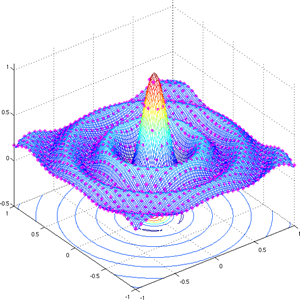
\includegraphics[scale=0.25]{../../img/sinc.PNG}}

\section{多项式系数}
\label{sec:org02149d0}


一个有意思的问题:把\(n\)个不同的元素分成\(r\)组,每组分别有\(n_{1},\ldots ,n_{r}\)个元素,\(\sum_{i=1}^{r}n_{i} = n\),一共有多少种方法?

要解决这个问题,我们可以把这个问题分成多个步骤:
\begin{enumerate}
\item 在\(n\)个元素中选择\(n_{1}\)个作为第一组,一共有\(\binom{n}{n_{1}}\)中选择方法;
\item 在剩下的\(n-n_{1}\)个元素中选择\(n_2\)个作为第二组,一共有\(\binom{n-n_{1}}{n_{2}}\)中选择方法;
\item 在剩下的\(n-n_{1}-n_{2}\)个元素中选择\(n_{3}\)个作为第三组,一共有\(\binom{n-n_{1}-n_{2}}{n_{3}}\)中选择方法;
\item 依次类推,经过了\(n_{r}-1\)步,从剩下的\(n-n_{1} - \ldots n-n_{r-1}\)个元素中选取\(n_{r}\)个元素作为第\(n_{r}\)组,一共有\(\binom{n- n_{1} - \ldots - n_{r-1}}{n_{r}}\)
\end{enumerate}

综上,可能的分法一共有:
\begin{eqnarray}
\label{eq:3}
&&  \binom{n}{n_{1}}\binom{n-n_{1}}{n_{2}}\binom{n-n_{1}-n_{2}}{n_{3}} \ldots \binom{n- n_{1} - \ldots - n_{r-1}}{n_{r}}\\
&=& \frac{n!}{(n-n_{1})!n_{1}!} \cdot \frac{(n-n_{1})!}{(n-n_{1}- n_{2})!n_{2}!} \ldots \frac{(n-n_{1} - \ldots - n_{r-1})!}{0!n_{r}!}\\
&=& \frac{n!}{n_{1}!n_{2}!\ldots n_{r}!}
\end{eqnarray}

从上面的计算过程我们可以看到,这个式子和 \href{afcp-combinatorial-analysis.org}{排列组合分析一文} 中的式1完全一样。因此我们可以考虑:

\textbf{排列} 假设有\(n\)个互不相同的元素,则一共有\(n!\)个排列结果。如果这\(n\)个元素,其中\(n_{1}\)个彼此相同,另\(n_{2}\)个彼此相同,依次类推,\(n_{r}\)个也彼此相同,那么一共排列的个数为:
\begin{equation}
\label{eq:4}
\frac{n!}{n_{1}!n_{2}!\ldots n_{r}!}
\end{equation}

如此,我们可以把这\(n\)个元素都打上标记,其中有\(n_{1}\)个\(1\),有\(n_{2}\)个\(2\),等等等等,有\(n_{r}\)个\(r\),则我们把这些标记做个排列,每次排列后,把标记为\(1\)位置上的\(n_{1}\)个元素归类为\(n_{1}\),把标记\(2\)对应的\(n_{2}\)个元素归类为第二组,依次类推把标记\(r\)对应的元素归类为第\(r\)组。那么将\(n\)个元素分成大小为\(n_{1},n_{2},\ldots ,n_{r}\)这样不同\(r\)组的分法数量,与\(n\)个值中,\(n_{1}\)相同,\(n_{2}\)相同,等等,\(n_{r}\)相同的排列数是相等的,这等于:\[\frac{n!}{n_{1}!n_{2}!n_{3}!\ldots n_{r}!} \]

\begin{definition}
如果\(n_{1} + n_{2} + \ldots + n_{r} = n\),则定义:\(\binom{n}{n_{1},n_{2},\ldots ,n_{r}}\)为:\[\binom{n}{n_{1},\ldots ,n_{r}} = \frac{n!}{n_{1}!\ldots n_{r}!}\] 因此,\(\binom{n}{n_{1},n_{2},\ldots ,n_{r}}\) 表示吧\(n\)个不同的元素分成大小为\(n_{1},\ldots ,n_{r}\)的\(r\)个不同组的组合数。
\end{definition}
\section{多项式定理}
\label{sec:org9f0b56a}


\begin{theorem}
\begin{equation}
\label{eq:5}
(x_{1} + \ldots + x_{r})^{n} = \sum_{\substack{ (n_{1},\ldots ,n_{r}) \\ n_{1} + \ldots + n_{r} = n }} \binom{n}{n_{1},n_{2},\ldots ,n_{r}} x_{1}^{n_{1}}x_{2}^{n_{2}}\ldots x_{r}^{n_{r}}
\end{equation}
上式的求和号是对满足\(n_{1}+ \ldots + n_{r} = n\)的所有非负整数向量\((n_{1},\ldots ,n_{r})\)求和。
\end{theorem}

\begin{proof}
我们知道\((x_{1} + \ldots + x_{r})^{n}\)结果是\(k\)个元素之和,\(k\)是\(n_{1}+\ldots +n_{r} = 0\)具有非负整数解的个数。每个元素的是\(n\)次项。每一个\(n\)次项中的\(x_{1},x_{2},\ldots ,x_{r}\)的幂次之和是\(n\),因此上述定理成立。
\end{proof}
\section{淘汰赛场次问题}
\label{sec:orge7d69fe}


\begin{instance}
假设有\(n\)名选手进行淘汰赛,\(n\)是\(2^{m}\)。这\(n\)名选手被分成\(n/2\)组,每组都要相互比赛,每一场比赛的失败者将被淘汰而胜者进入下一轮,这个过程持续到只有一名选手留下。假设我们有一场淘汰赛,其中有\(8\)名选手。
\begin{enumerate}
\item 第一轮之后有多少种可能的结果?
\item 这场淘汰赛有多少种可能的结果?其中每个结果包含了所有轮次的完整信息。
\end{enumerate}
\end{instance}

\begin{answer}
首先,对于第一个问题,我们把\(8\)个人分为\(4\)组,每组\(2\)个这样的分法有\(\binom{8}{2,2,2,2}= \frac{8!}{2^{4}}\)种分法,然后,当这四组没有顺序的差别时,\(\frac{8!}{2^{4}\times 4!}\)种分法。对于比赛结果每一组都有两种所以一共有\(\frac{8!\times 2^{4}}{2^{4} \times 4!} = \frac{8!}{4!}\)

对于第一个问题,我们还有另外的解法。首先选出\(4\)名胜利者一共有\(\binom{8}{4}\)种方法,然后为这四名胜利者配对一个失败者,一共有\(4!\)种方法。所以结合这两步,一共有\(\binom{8}{4}\times 4! =\frac{8!}{4!}\)种方法。

第二种方法是第一种方法的扩展,则有:第二轮的结果有\(\frac{4!}{2!}\),第三轮的结果有\(\frac{2!}{1!}\),所以一共有\(\frac{8!}{4!}\times \frac{4!}{2!} \times \frac{2!}{1!} = 8!\)

我们可以进一步考虑,是不是淘汰赛的结果和\(1,\ldots ,n\)排列之间存在一一对应的关系,所以结果才是\(n!\). 我们可以这样理解,对于淘汰赛而言其结果有一个排名,从第\(n\)名到第\(n\)名,所以一共有\(n!\)种排名。
\end{answer}
\section{方程整数解个数}
\label{sec:orgc81dcf2}


在上面多项式定理中,对于多项式展开的和中元素个数\(K\),我们没有给出一个解析解。现在我们尝试推出\(K\)的闭式解。假设\(n=n_{1} + \ldots + n_{r}\),则要计算可能的非负整数向量\((n_{1},\ldots ,n_{r})\),我们考虑有\(n\)个连续的\(0\)排成一行:
\[0\quad 0\quad \cdots \quad 0\]
从\(n-1\)个相邻的\(0\)的间隔中选出\(r-1\)个间隔的每一个方式对应等式:\[n=n_{1} + \ldots + n_{r}\]一个正整数解:令\(n_{1}\)等于第一个被选择的间隔之前的\(0\)的个数,\(x_{2}\)等于第一个和第二被选择的间隔之间的\(0\)的个数,依次类推,\(n_{r}\)等于最后一个被选的间隔后面的\(0\)的个数。于是:
\begin{theorem}
共有\(\binom{n-1}{r-1}\)个不同的正整数向量\((n_{1},n_{2},\ldots ,n_{r})\)满足:
\begin{equation}
\label{eq:6}
n_{1} + n_{2} + \ldots n_{r} = n, n_{i} > 0, i = 1,\ldots ,r
\end{equation}
\end{theorem}
为了得到非负整数解的个数,注意\(x_{1} + \ldots +x_{r} = n\)的非负整数解的个数和\(y_{1}+ \ldots y_{r} = n+r\)的正整数解的个数是相同的(令\(y_{i} = x_{i} + 1,i = 1,\ldots ,r\)),于是:
\begin{theorem}
共有\(\binom{n+r-1}{r-1}\)个不同的非负整数向量\((x_{1},\ldots ,x_{r})\)满足:
\begin{equation}
\label{eq:7}
x_{1} + x_{2} +\ldots + x_{r} = n
\end{equation}
\end{theorem}
\section{一个应用}
\label{sec:orgf74b476}


我们再来讨论天线有效问题:有\(n\)个天线,其中\(m\)个是不可分辨的失效天线,令\(n-m\)个天线也是不可分辨但是有效的。现在要求排成一排且没有相邻的两个失效天线的可能排列数。

我们可以假设\(n-m\)个有效的天线排成一排,一共有\(n-m+1\)个间隔,根据题目要求每个间隔中最多放一根失效天线,所以问题就变成从\(n-m+1\)个间隔中找出\(m\)个位置放置失效天线。即有\(\binom{n-m+1}{m-1}\)种天线排列方法。

另外我们还可以先把\(m\)个失效的天线排成一排,一共有\(m+1\)个间隔,我们要把这\(n-m\)个有效天线放到\(m+1\)个间隔中。因此放置的天线排列数是\[n_{1} + \ldots + n_{m+1} = n-m\]的解的个数,满足\(n_{1} \leq 0, n_{i} > 0, i=2,\ldots ,m;\) \(x_{m+1} \leq 0\)。令\(y_{1} = x_{1} + 1;y_{i} = x_{i},i=2,\ldots ,m;y_{m+1} = x_{m+1} + 1\),所以这个问题等于:
\begin{equation}
\label{eq:8}
y_{1} + \ldots + y_{m+1} = n-m+2
\end{equation}
的正整数向量的个数,因此一共有\(\binom{n-m+1}{m}\)中方法,和我们之前得出的结果一样。

现在来考虑每两个失效天线之间至少有\(2\)个有效天线这种情况的排列数,结果为如下方程的解的个数:
\[x_{1} + \ldots + x_{m+1} = n-m,x_{1}\leq 0 ;x_{m+1}\leq 0 ;x_{i}\geq 2,i=2,\ldots ,m\]
令\(y_{1} = x_{1} + 1,y_{m+1} = x_{m+1} + 1;y_{i} = x_{i}-1,i=2,\ldots ,m\),则问题变为:
\[y_{1} + \ldots + y_{m+1} = n-m +2 -  (m-1)\]
有正整数解的个数。所以一共有\(\binom{n-2m +2}{m}\)个天线配置方式。
\end{document}
